\documentclass[logo,reportComp]{thesis}
\usepackage[cpp,linenum]{mypackage}

\usetikzlibrary{automata,backgrounds,fit,shapes,positioning}

\tikzset{->, % makes the edges directed
>=stealth, % makes the arrow heads bold
node distance=2cm, % specifies the minimum distance between two nodes. Change if necessary.
every state/.style={thick, fill=gray!10}, % sets the properties for each 'state' node
}

\title{编译原理期末大作业}
\subtitle{正则表达式等价性}
\school{数据科学与计算机学院}
\author{陈鸿峥}
\classname{17大数据与人工智能}
\stunum{17341015}
\headercontext{编译原理期末大作业}

\begin{document}

\maketitle
\tableofcontents

\newpage

\section{实验目的}
对于两个正则表达式$r$和$s$,判断这两个正则表达式的关系。
正则表达式$r$和$s$的关系有4种:
\begin{enumerate}
\item $r$和$s$等价,即$r$描述的语言和$s$描述的语言相等;
\item $r$描述的语言是$s$描述的语言的真子集;
\item $s$描述的语言是$r$描述的语言的真子集;
\item 非上述情况。
\end{enumerate}
正则表达式的字符集为小写字母\verb'a'-\verb'z',\verb'|'号表示或者,\verb'*'号表示闭包,\verb'?'表示出现$0$或$1$次,$+$表示至少出现一次,大写字母$E$表示epsilon(空串)。

编写一个C++程序,实现上述功能。

\textbf{输入格式:}\par
第一行是测试数的组数$T$。
接下来的$T$行,每行是两个正则表达式$r$和$s$,每个正则表达式只含\verb'a'-\verb'z',\verb'|',\verb'*',\verb'?',\verb'+',\verb'(',\verb')',\verb'E'。
两个正则表达式之间用空格分开。

\textbf{输出格式:}\par
输出有$T$行。
对于每组数据,如果$r$和$s$等价,输出\verb'=';
如果$r$是$s$的真子集,输出\verb'<';
如果$s$是$r$的真子集,输出\verb'>';
非上述情况,输出\verb'!'。

\textbf{提交内容:}
\begin{enumerate}
	\item 能在Linux下或在Windows的Dev C++下编译运行的C++源程序;
	\item 实验报告,包括算法描述,和你的测试用例,及测试结果。
\end{enumerate}

% 提交截止日期:7.25

\section{算法原理}
本次实验主要分为以下几个部分(如图\ref{fig:flowgraph}所示),正则表达式读入、字符串预处理、中缀转后缀表示、正则表达式转NFA、NFA转DFA、DFA最小化、DFA等价性判断,下文会依次阐述算法细节。
\begin{figure}[H]
\centering
\includegraphics[width=\linewidth]{fig/regex-flowgraph.pdf}
\caption{算法核心流程}
\label{fig:flowgraph}
\end{figure}

\subsection{字符串预处理}
最开始读入的正则表达式并不方便后续的操作,因此需要对其进行一些预处理。
这里包括加法符号替代和连接符号插入两项预处理。

\subsubsection{加法符号替代}
加法符号\verb'+'用来表示前文的符号出现至少一次,这并非最简正则所支持的语法,因此我们需要对其进行替代。
注意到
\begin{center}
\verb'R+' $\iff$ \verb'RR*'
\end{center}
因此可以将\verb'R+'替换成用星号表示的形式。

需要注意\verb'R'也是一个正则表达式,故需要确定其包含的内容,然后才可以做拷贝替换。
这里我直接在输入的正则字符串上进行操作:
\begin{itemize}
	\item 若\verb'R'就是单一字母(\verb'a-z'),那么直接在其后面添加\verb'R*'。
	\item 若\verb'R'为括号包围的正则表达式,则需要将括号包围的内容整份进行拷贝。
	具体实现可用栈维护括号的位置,遇到左括号则将其下标进栈,遇到右括号弹出栈顶的下标;如果右括号的下一符号为\verb'+',则将当前下标与栈顶下标这一区间的字符串进行拷贝,附加在当前字符的右侧,并添加\verb'*'作结。
\end{itemize}

一个例子如下
\begin{center}
\verb'((x|y)+)+' 展开后为 \verb'((x|y)(x|y)*)((x|y)(x|y)*)*'
\end{center}
只有正确使用栈操作才能够正确处理上述\textbf{嵌套括号}的情况。

完整实现见源码的\verb'substitute_plus'函数。

\subsubsection{连接符号插入}
接下来一步则是对连接符进行插入。
由于原有的正则表示式都是默认省略连接符,这会给后续的分析转换带来麻烦,因此这一步则是将省略的这些连接符进行插入,这里用\verb'.'代表连接符。

由于只需判断当前字符与下一字符的关系,这里只给出一个例子以示说明,完整实现请见\verb'insert_concat'函数。
\begin{center}
\verb'b*a*b?a*' 变为 \verb'b*.a*.b?.a*'
\end{center}

\subsection{中缀转后缀表示}
处理完加号和连接符后,即可将中缀的正则表达式转换为后缀形式表达,这将方便后续NFA转换的处理。

算法流程如下,利用一个算子栈进行状态维护:
\begin{enumerate}
	\item 从左到右遍历中缀表达式
	\item 如果当前字符是
	\begin{itemize}
		\item 字母(\verb'a-z'或\verb'E'),则将其添加入输出中
		\item 左括号\verb'(',将其推入栈中
		\item 右括号\verb')',将栈顶的符号依次弹出,直至遇见左括号(左括号也要弹出)
		\item 算子,先将栈顶\textbf{优先级比该算子高}的符号依次弹出,再将当前算子推入栈中
	\end{itemize}
	\item 循环以上过程,直至字符串遍历完
	\item 将栈顶剩余的符号全部弹出
\end{enumerate}

完整代码请见\verb'infix2postfix'函数。

\subsection{正则表达式转NFA}
正则表达式转NFA即课本3.7.4节所述的Thompson算法,按照以下方式可以进行构造。

\begin{enumerate}
	\item 奠基
\begin{itemize}
\item 对于表达式$\epsilon$(即输入为\verb'E'),构建NFA
\begin{center}
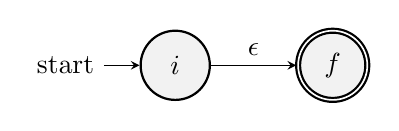
\begin{tikzpicture}
\node[state, initial] (1) {$i$};
\node[state, accepting, right of=1] (2) {$f$};
\draw (1) edge[above] node{$\epsilon$} (2);
\end{tikzpicture}
\end{center}

\item 对于任意子表达式$a\in\Sigma$,构建NFA
\begin{center}
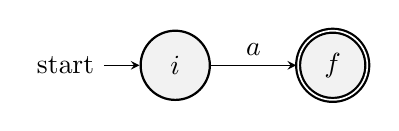
\begin{tikzpicture}
\node[state, initial] (1) {$i$};
\node[state, accepting, right of=1] (2) {$f$};
\draw (1) edge[above] node{$a$} (2);
\end{tikzpicture}
\end{center}
\end{itemize}
	\item 推论
\begin{itemize}
\item $r=s|t$,取并集
\begin{center}
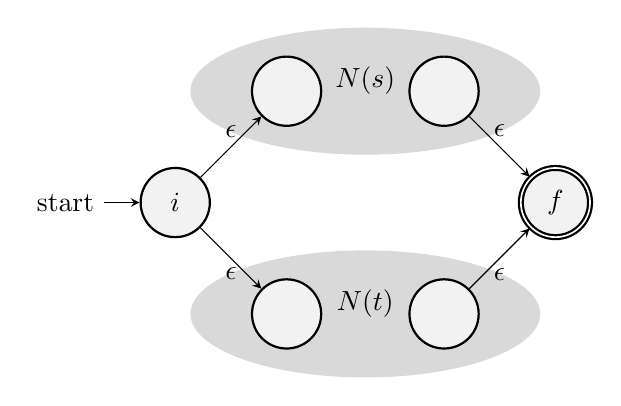
\begin{tikzpicture}
\node[state, initial] (1) {$i$};
\node[state, above right of=1] (2) {};
\node[state, below right of=1] (3) {};
\node[state, right of=2] (4) {};
\node[state, right of=3] (5) {};
\node[state, accepting, below right of=4] (6) {$f$};
\draw (1) edge[above] node{$\epsilon$} (2)
(1) edge[below] node{$\epsilon$} (3)
(4) edge[above] node{$\epsilon$} (6)
(5) edge[below] node{$\epsilon$} (6);
\begin{pgfonlayer}{background}
\node[fit=(2)(4), fill=gray!30, ellipse] {$N(s)$};
\node[fit=(3)(5), fill=gray!30, ellipse] {$N(t)$};
\end{pgfonlayer}
\end{tikzpicture}
\end{center}

\item $r=st$,取连接
\begin{center}
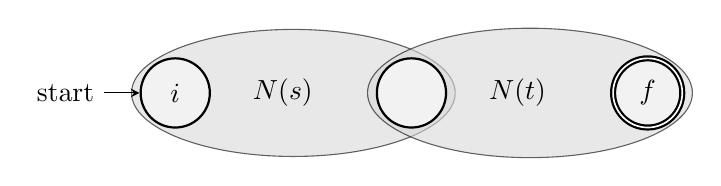
\begin{tikzpicture}[node distance=3cm,
	FIT/.style args = {#1/#2/#3}{ellipse, fill=#1, inner xsep=#2, fit=#3}]
\node[state, initial] (1) {$i$};
\node[state, right of=1] (2) {};
\node[state, accepting, right of=2] (3) {$f$};
\node[right=0.41cm of 1] {$N(s)$};
\node[right=0.41cm of 2] {$N(t)$};
% \draw[draw=gray!30,arrows={->[gray!30]}] (1) edge[above] node{$N(s)$} (2);
% \draw[draw=gray!30,arrows={->[gray!30]}] (2) edge[above] node{$N(t)$} (3);
\begin{pgfonlayer}{background}
\node[FIT=gray!30/-5mm/(1)(2), draw=black, opacity=0.6] {};
\node[FIT=gray!30/-5mm/(2)(3), draw=black, opacity=0.6] {};
\end{pgfonlayer}
\end{tikzpicture}
\end{center}

这里为方便程序实现,采用了如下的构造方式。
\begin{center}
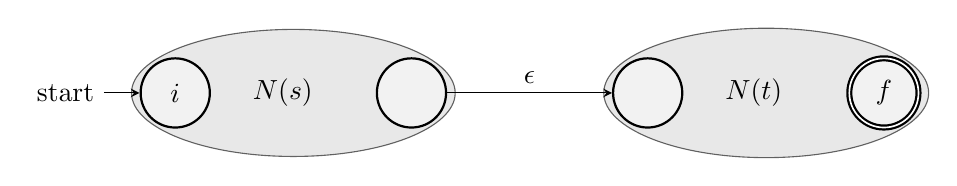
\begin{tikzpicture}[node distance=3cm,
	FIT/.style args = {#1/#2/#3}{ellipse, fill=#1, inner xsep=#2, fit=#3}]
\node[state, initial] (1) {$i$};
\node[state, right of=1] (2) {};
\node[state, right of=2] (4) {};
\node[state, accepting, right of=4] (3) {$f$};
\node[right=0.41cm of 1] {$N(s)$};
\node[right=0.41cm of 4] {$N(t)$};
\draw (2) edge[above] node{$\epsilon$} (4);
% \draw[draw=gray!30,arrows={->[gray!30]}] (1) edge[above] node{$N(s)$} (2);
% \draw[draw=gray!30,arrows={->[gray!30]}] (2) edge[above] node{$N(t)$} (3);
\begin{pgfonlayer}{background}
\node[FIT=gray!30/-5mm/(1)(2), draw=black, opacity=0.6] {};
\node[FIT=gray!30/-5mm/(4)(3), draw=black, opacity=0.6] {};
\end{pgfonlayer}
\end{tikzpicture}
\end{center}

\item $r=s^*$,Kleene闭包
\begin{center}
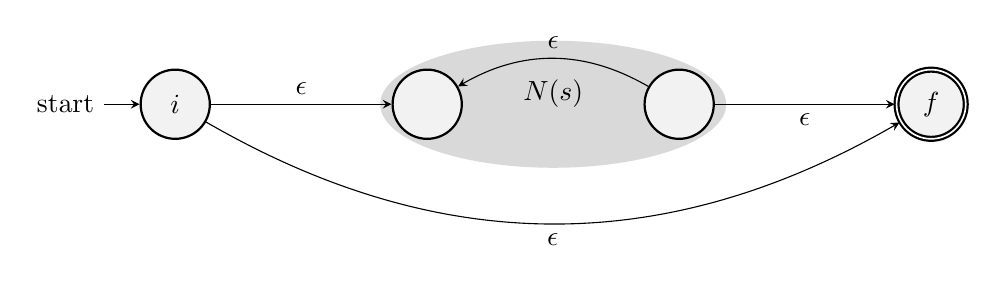
\begin{tikzpicture}[node distance=3.2cm,
	FIT/.style args = {#1/#2/#3}{ellipse, fill=#1, inner xsep=#2, fit=#3}]
\node[state, initial] (1) {$i$};
\node[state, right of=1] (2) {};
\node[state, right of=2] (3) {};
\node[state, accepting, right of=3] (4) {$f$};
\draw (1) edge[above] node{$\epsilon$} (2)
(1) edge[bend right, below] node{$\epsilon$} (4)
(3) edge[above, bend right] node(e){$\epsilon$} (2)
(3) edge[below] node{$\epsilon$} (4);
\begin{pgfonlayer}{background}
\node[FIT=gray!30/-5mm/(2)(3)] {$N(s)$};
\end{pgfonlayer}
\end{tikzpicture}
\end{center}

\item $r=s?$,这是本问题新加的语法,代表0个或1个输入,相当于$r=\epsilon|s$,故只需对并集自动机的构造进行适当修改即可。
\begin{center}
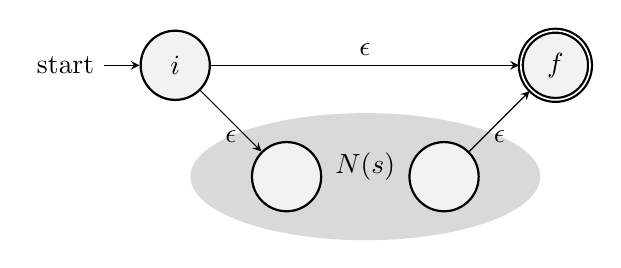
\begin{tikzpicture}
\node[state, initial] (1) {$i$};
\node[state, below right of=1] (2) {};
\node[state, right of=2] (3) {};
\node[state, accepting, above right of=3] (4) {$f$};
\draw (1) edge[below] node{$\epsilon$} (2)
(3) edge[below] node{$\epsilon$} (4)
(1) edge[above] node{$\epsilon$} (4);
\begin{pgfonlayer}{background}
\node[fit=(2)(3), fill=gray!30, ellipse] {$N(s)$};
\end{pgfonlayer}
\end{tikzpicture}
\end{center}

\end{itemize}
\end{enumerate}

具体实现上需要创建一个NFA结点类,存储其结点编号、状态、出边,定义如下。
\lstinputlisting[language=c++,firstline=13,lastline=23]{../main.cpp}
并用一个栈对NFA结点进行维护,每次从后缀表达式中读取一个符号,从栈顶弹出对应$N(s)$和$N(t)$的入口结点及出口结点,并按照以上构造方式,创建新的$i$和$f$结点,连接好对应边后,将$i$和$f$推入栈顶。

完整代码见\verb'regex2nfa'函数。

\subsection{NFA转DFA}
NFA转DFA的算法参见课本第3.7.1节,即子集构造算法,这里需要以下几个操作。
关于集合的操作均采用C++的\verb'<set>'标准库进行实现,而计算闭包则是通过递归深度优先搜索(DFS)实现。
\begin{center}
\begin{tabular}{|c|c|}\hline
操作 & 描述\\\hline
$\epsilon$-$closure(s)$ & 从状态$s$能够通过$\epsilon$边转换的集合(包括自己的状态)\\\hline
$\epsilon$-$closure(T)$ & $\bigcup_{s\in T}\epsilon$-$closure(s)$\\\hline
$move(T,a)$ & 从$s\in T$中的状态通过输入符号$a$进行转换\\\hline
\end{tabular}
\end{center}

同时,构造DFA结点类,存储其结点编号、状态及出边,定义如下。
\lstinputlisting[language=c++,firstline=25,lastline=36]{../main.cpp}
注意到DFA中就没有$\epsilon$边了。

具体算法参见图\ref{fig:nfa2dfa},其中状态的访问用队列\verb'queue'维护,状态标记用集合\verb'set'维护,状态转移用映射\verb'map'维护。
\begin{figure}[H]
\centering
\includegraphics[width=0.9\linewidth]{fig/nfa2dfa.jpg}
\caption{子集构造算法}
\label{fig:nfa2dfa}
\end{figure}

完整代码见\verb'nfa2dfa'函数,需要注意在计算闭包构造新结点的同时也要记录开始状态和接受状态。

\subsection{DFA最小化}
由于每个正则表达式对应的最小化DFA是唯一的,因此可以通过最小化DFA的方式来判断两个正则表达式之间的关系,这里采用课本3.9.6节的Hopcroft划分算法。
这一部分算是本次实验所有算法中最难实现的一个,需要考虑到非常多的细节。

算法流程如下:
\begin{enumerate}
	\item 开始初始划分为$\prod$,所有接受状态$F$为一个组,该集合的补为另一个组$S-F$(注意有可能所有状态均为接受状态,那么$S-F=\varnothing$),将这两个组推入队列中
	(在具体实现上我并没有将所有划分用统一的数据结构进行存储,而是在原有每个DFA结点下添加\verb'group'成员进行标记)
	\item 若组队列非空,则弹出头部的组
	\begin{itemize}
		\item 若该组只有一个状态,则不需划分
		\item 若改组有多个状态,并且存在两个状态对于相同符号的出边落在不同的组,那么这两个状态需要被划分为不同的组(具体实现上采用\verb'map<int,vector<int>>'对状态进行维护,考察每个DFA结点对相同符号的出边,目标结点的组标号为\verb'map'的key,而value则是组内的状态编号),将划分后的新组重新加入队列
	\end{itemize}
	\item 对组编号进行重新分配及映射,为每个组挑选旧DFA中的标志结点,并创建新的DFA结点,将新的结点按照旧的连边关系建图,生成最终最小化DFA
\end{enumerate}

完整代码见\verb'minimize_dfa'函数,这里在划分组时需要小心一些出边并不完全的DFA。
一个简单的例子即\verb'a',生成的DFA如下图所示。
\begin{center}
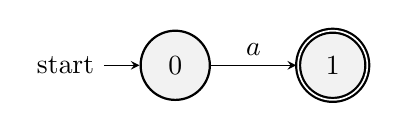
\begin{tikzpicture}
\node[state, initial] (1) {$0$};
\node[state, accepting, right of=1] (2) {$1$};
\draw (1) edge[above] node{$a$} (2);
\end{tikzpicture}
\end{center}
该DFA的接受结点即没有任何的出边,这在访问时需要特别小心。
比如在分组时就会将这些访问不到出符号的结点的出结点的组别设为$-1$。

在具体实现上\verb'map'不能直接通过\verb'[]'进行读取,哪怕没有该元素,也会读出值造成错误;
故应该用\verb'.count(c)'判断\verb'c'元素是否存在映射中,并用\verb'.at(c)'来读出\verb'c'的内容。

\subsection{DFA等价性判断}
最后一步则是进行DFA等价性的判断。
注意到每个正则表达式都可以对应一个DFA,而两个DFA $R$和$S$之间的关系只会有四种情况,可以考察原DFA与补DFA的交关系来判断原始两个DFA之间的包含关系,如图\ref{fig:dfa-test}所示。
\begin{itemize}
	\item $R$等价于$S$:$R\cap\bar{S}=\varnothing\land \bar{R}\cap S=\varnothing$
	\item $R$含于$S$:$R\cap\bar{S}=\varnothing\land \bar{R}\cap S\ne\varnothing$
	\item $S$含于$R$:$R\cap\bar{S}\ne\varnothing\land \bar{R}\cap S=\varnothing$
	\item 其他关系:$R\cap\bar{S}\ne\varnothing\land \bar{R}\cap S\ne\varnothing$
\end{itemize}
其中这里$\bar{\cdot}$代表DFA的补,即将所有接受状态变为非接受状态,非接受状态变为接受状态。

\begin{figure}[H]
\centering
\includegraphics[width=\linewidth]{fig/regex-dfa-test.pdf}
\caption{DFA关系的四种情况}
\label{fig:dfa-test}
\end{figure}

所以只需求两个DFA是否\textbf{相交}即可,具体方法是对两个DFA同时从开始状态进行模拟。
如果模拟到两个状态$s1$和$s2$都为接受态,意味着有一个字符串可以同时被两个DFA/正则表达式所匹配,即两个DFA相交;
如果对于所有字符串,都没有办法使两个DFA同时到达接受态,则这两个DFA不相交。

具体实现采用递归的DFS。
为防止陷入死循环,开设一个\verb'visited'二维数组记录两个DFA访问过的状态。
算法流程如下,函数为\verb'intersection(s1,s2,dfa1,dfa2,visited)'。
\begin{enumerate}
	\item 设置状态$(s1,s2)$为已访问
	\item 若$(s1,s2)$均为接受态,返回真
	\item 对于每一个输入符号
	\begin{itemize}
		\item 求两个状态机在$(s1,s2)$下的状态转移,新的状态为$(o1,o2)$
		\item 若$(o1,o2)$未访问且\verb'intersection(o1,o2,dfa1,dfa2,visited)'为真,返回真
	\end{itemize}
	\item 若所有输入符号都没返回真,则返回假
\end{enumerate}

有了求交的算法就可以通过执行两次交判断语句来得到两个正则表达式的关系,即$R$与$\bar{S}$求交,$S$与$\bar{R}$求交。
因此还需要有一个辅助函数来对DFA进行求反。
由于之前已经创建了\verb'DFA_Node'的类,故求反只需将每个DFA的结点由接受态改为非接受态,非接受态改为接受态。

这里还需注意对于DFA的某些状态,可能没有对所有输入符号都有出边,这在模拟DFA时可能会出现错误。
对于这种情况,可以假设有一个冗余结点来接收这些非法输入。
如对于\verb'a'的DFA来说,右侧结点已经无法再接收其他符号,那么为保持每个结点输入符号都存在,可以添加多一个非接受态结点用以作为输出(即黑洞结点,只进不出),如下图所示。
\begin{center}
\begin{tabular}{cc}
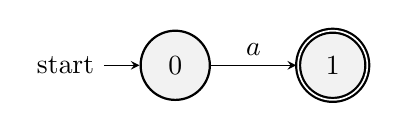
\begin{tikzpicture}
\node[state, initial] (1) {$0$};
\node[state, accepting, right of=1] (2) {$1$};
\draw (1) edge[above] node{$a$} (2);
\end{tikzpicture}&
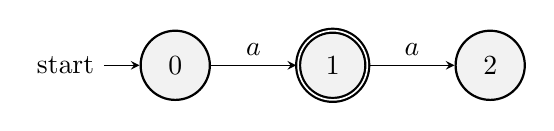
\begin{tikzpicture}
\node[state, initial] (1) {$0$};
\node[state, accepting, right of=1] (2) {$1$};
\node[state, right of=2] (3) {$2$};
\draw (1) edge[above] node{$a$} (2);
\draw (2) edge[above] node{$a$} (3);
\end{tikzpicture}
\end{tabular}
\end{center}

完整代码可见\verb'judge'函数。

\section{实验结果}
已在Sicily上验证通过。

\appendix
\appendixconfig
\section{完整源码}
\lstinputlisting[language=c++,basicstyle=\footnotesize]{../main.cpp}
\lstinputlisting[language=c++,basicstyle=\footnotesize]{../utils.h}
\lstinputlisting[language={[gnu] make},basicstyle=\footnotesize]{../Makefile}

\section{测试数据}
\begin{center}
\begin{tabular}{|c|c|c|}\hline
\textbf{regex1} & \textbf{regex2} & \textbf{output}\\\hline
\verb'((E|a)b*)*' & \verb'(a|b)*' & \verb'='\\\hline
\verb'b*a*b?a*' & \verb'b*a*ba*|b*a*' & \verb'='\\\hline
\verb'b*a*b?a*' & \verb'(b*|a*)(b|E)a*' & \verb'>'\\\hline
\verb'(c|d)*c(c|d)(c|d)' & \verb'(c|d)*d(c|d)(c|d)' & \verb'!'\\\hline
\verb'x+y+z+' & \verb'x*y*z*' & \verb'<'\\\hline
\verb'a' & \verb'a+' & \verb'<'\\\hline
\verb'(a|b)*abb' & \verb'(a|b)*abbb*' & \verb'<'\\\hline
\verb'(a|b)*c+(d|e)?' & \verb'(a|b)*cd' & \verb'>'\\\hline
\verb'((x|y)+)+' & \verb'(x|y)+(y+b*)*' & \verb'<'\\\hline
\end{tabular}
\end{center}

\end{document}

% infix2postfix, https://www.geeksforgeeks.org/stack-set-2-infix-to-postfix/
% nfa2regex, https://github.com/Ronan-H/regex-nfa-builder/blob/master/nfa_utils.py
% test isomorphism, https://stackoverflow.com/questions/6905043/equivalence-between-two-automata
% https://cyberzhg.github.io/toolbox/min_dfa
% https://runestone.academy/runestone/books/published/pythonds/BasicDS/InfixPrefixandPostfixExpressions.html
% http://www.cppblog.com/woaidongmao/archive/2010/09/05/97541.html